\documentclass[11pt,a4paper]{article}
\usepackage[margin=2cm]{geometry}
\usepackage[T1]{fontenc}
\usepackage{lmodern}
\usepackage{microtype}
\usepackage{amsmath,amssymb}
\usepackage{graphicx}
\usepackage{booktabs}
\usepackage{float}
\usepackage[font=small,skip=4pt]{caption}
\usepackage{subcaption}
\usepackage{xcolor}
\usepackage{tikz}
\usetikzlibrary{arrows.meta,positioning}
\usepackage[hidelinks]{hyperref}

\graphicspath{{figures/}}
\definecolor{ours}{HTML}{2A78D6}
\definecolor{muted}{HTML}{52514E}
\setlength{\parskip}{4pt}
\setlength{\parindent}{0pt}
\setlength{\textfloatsep}{8pt}
\setlength{\floatsep}{6pt}

% "In short" box: one takeaway per section
\newcommand{\inshort}[1]{\par\smallskip\noindent\fcolorbox{ours!45}{ours!6}{\parbox{\dimexpr\linewidth-2\fboxsep-2\fboxrule}{\small\textbf{In short:} #1}}\par\smallskip}

\title{\vspace{-1.2cm}Negotiated Local Plan Repair for Multi-Robot Warehouse Pathfinding}
\author{\begin{tabular}{ccc}Sreenitya Thatikunta & Arpita Deshmukh & Prajna Agrawal\\ B23CS1072 & B23CM1007 & B23CS1054\end{tabular}}
\date{\vspace{-0.6cm}}

\begin{document}
\maketitle
\vspace{-0.5cm}

\section{The problem}
A team of robots works in a warehouse. The floor is a grid of square cells. In each time step,
every robot either moves one cell (up, down, left or right) or waits. Each robot has
\textbf{3 tasks}: go to a shelf, pick up an item, carry it to a delivery station. After its last
task it drives back to its own parking spot (its \emph{dock}). Two robots may never be in the same
cell at the same time, and may never swap cells with each other in one step.

Before starting, the robots plan collision-free paths. Then, while they follow these paths,
\textbf{things go wrong}:
\begin{itemize}\setlength{\itemsep}{1pt}
  \item a robot \textbf{breaks down} (for 5--20 steps, or for good);
  \item a cell gets \textbf{blocked} (for 10--40 steps, or for good);
  \item a robot gets an \textbf{emergency task} that it must do first, with a deadline.
\end{itemize}
The robots must then \textbf{repair} their plans. The rules of the assignment are: robots fix
things by talking to nearby robots; we must not re-plan the whole fleet from scratch; and we
should change \textbf{as few robots' plans as possible}.

\textbf{Our warehouse.} The map is $18\times33$ cells: 25 shelf blocks with one-cell-wide aisles
between them, 150 pickup cells next to the shelves, 14 delivery stations on the side walls and 58
docks on the top and bottom walls (Figure~\ref{fig:demo} on the last page shows it).

\begin{table}[H]
\centering\small
\caption{Key terms used in this report.}
\label{tab:terms}
\begin{tabular}{p{0.24\linewidth}p{0.70\linewidth}}
\toprule
\textbf{Plan} & The list of cells a robot will visit, one per time step. \\
\textbf{Disruption} & A breakdown, a blocked cell or an emergency task that happens while robots move. \\
\textbf{Plan repair} & Fixing the plans after a disruption, without starting over. \\
\textbf{Altered robots} & How many robots had to change their plan because of one disruption. \textbf{Lower is better.} \\
\textbf{Total time (SoC)} & ``Sum of costs'': add up the time step at which each robot finishes its tasks. \textbf{Lower is better.} \\
\textbf{Extra steps} & Total time with disruptions minus total time of the original, undisturbed plan. \\
\textbf{Obstacle density} & How many cells get blocked during a run, as a share of all free cells (e.g.\ 5\%). \\
\textbf{Communication range} & Robots can only talk to robots within 6 cells of them. \\
\bottomrule
\end{tabular}
\end{table}

\section{Our approach}
\subsection*{Step 1: the initial plan}
We use \textbf{prioritized planning with Space-Time A*}. The robots plan \emph{one after another}
(the robot with the longest trip goes first). Space-Time A* is the A* shortest-path search, but
on cells \emph{and} time, so it can also decide to wait. Every finished plan is written into a
shared \textbf{reservation table}, like booking a cell in a calendar: ``cell (5,7) is taken by robot
3 at time 12''. Later robots simply plan around the bookings, so no two plans collide.

\subsection*{Step 2: repairing after a disruption}
When something goes wrong, only the robots whose plans are now broken are fixed, one at a time.
Each one climbs a \textbf{ladder of fixes}, from the fix that disturbs nobody else to fixes that
involve more robots (Figure~\ref{fig:protocol}). It stops at the first fix that is good enough.

\begin{enumerate}\setlength{\itemsep}{2pt}
  \item \textbf{Fix it alone (Tier 1).} The robot re-plans its own path and treats everyone else's
        plan as fixed. If this costs at most 4 extra steps, accept it. Only one plan changes.
  \item \textbf{Ask neighbours for help (Tiers 2--3).} The robot finds which nearby robots are in
        its way and asks a small group of them (1, then 2, then 3 robots) to re-plan together with
        it. It first asks within 6 cells, then within 12. If a helper is itself blocked, the helper
        may ask \emph{its} neighbours too (a \emph{chain}, at most 2 levels deep).
  \item \textbf{Re-plan a small local group (Tier 3b).} Only for urgent cases (an emergency robot,
        or a robot with no path at all): re-plan the robot together with up to 8 robots near it.
  \item \textbf{Detour or wait (Tier 4).} Otherwise the robot takes its long detour, or, if it has
        no path at all, waits where it is and tries again next step. If it has to wait for 10
        steps, it starts asking robots further away.
\end{enumerate}

\textbf{How a robot decides whether asking for help is worth it.} Every option gets a score:
\begin{center}
\fbox{\parbox{0.86\linewidth}{\centering \textbf{score} = extra steps for everyone involved \;+\; 3 for every other robot disturbed\\ \;+\; 10 if an emergency deadline is missed}}
\end{center}
Lower is better. A group fix is used only if it scores better than fixing it alone. The ``3 per
robot'' term is how we follow the rule ``change as few plans as possible'': disturbing another
robot is only worth it if it saves more than 3 steps.

\begin{figure}[H]
\centering
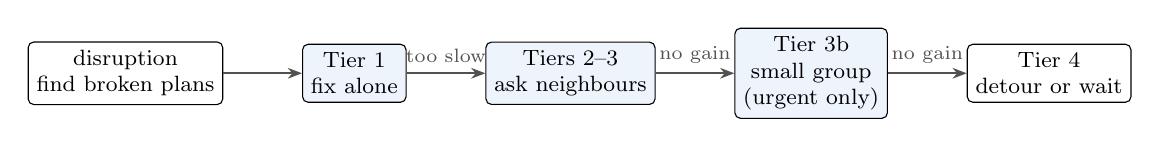
\begin{tikzpicture}[node distance=4mm and 10mm, every node/.style={font=\footnotesize},
  box/.style={draw, rounded corners=2pt, align=center, minimum height=7mm, inner sep=3pt},
  dec/.style={box, fill=ours!8}, arr/.style={-{Stealth[length=1.8mm]}, thick, muted}]
  \node[box] (d) {disruption\\find broken plans};
  \node[dec, right=of d] (t1) {Tier 1\\fix alone};
  \node[dec, right=of t1] (t2) {Tiers 2--3\\ask neighbours};
  \node[dec, right=of t2] (t3b) {Tier 3b\\small group\\(urgent only)};
  \node[box, right=of t3b] (t4) {Tier 4\\detour or wait};
  \draw[arr] (d) -- (t1);
  \draw[arr] (t1) -- node[above, font=\scriptsize]{too slow} (t2);
  \draw[arr] (t2) -- node[above, font=\scriptsize]{no gain} (t3b);
  \draw[arr] (t3b) -- node[above, font=\scriptsize]{no gain} (t4);
\end{tikzpicture}
\caption{The ladder of fixes. A robot only moves right when the current fix is not good enough,
so other robots are disturbed only when it really helps.}
\label{fig:protocol}
\end{figure}

\subsection*{What we compare against}
\begin{itemize}\setlength{\itemsep}{1pt}
  \item \texttt{local}: \textbf{our method} (the ladder above).
  \item \texttt{local-flat}: our first version, without chains, Tier 3b or deadlines.
  \item \texttt{solo}: only Tier 1 (no talking to other robots), to show what negotiation adds.
  \item \texttt{full}: re-plans \emph{every} robot from scratch after every disruption. The
        assignment forbids this for repair; we use it only as a reference point.
\end{itemize}

\inshort{robots plan one after another and book cells in a shared table. After a disruption,
each affected robot tries the cheapest fix first and only involves other robots when that saves
real time.}

\section{Experiments and results}
\textbf{How we tested.} We ran every setting \textbf{10 times} with different random seeds, and
gave all four methods exactly the same warehouse and the same disruptions. By default each run has
3\% obstacle density, 2 breakdowns and 2 emergencies. We varied the \textbf{number of robots}
(5 to 50) and the \textbf{obstacle density} (0\% to 15\%). We also ran tests with exactly
\textbf{one disruption}, to count how many plans a single disruption changes. In total: 1{,}700
runs. \textbf{No run had a collision}, and every task was completed (except one \texttt{solo} run,
Section~\ref{sec:fail}).

\begin{table}[H]
\centering\footnotesize\setlength{\tabcolsep}{4pt}
\caption{Main comparison at 20 and 50 robots (average of 10 runs, 12 disruptions per run). Read it
as: lower total time and fewer altered robots are better.}
\label{tab:agents}
\begin{tabular}{rlrrrr@{\hspace{2em}}rlrrrr}
\toprule
robots & method & total & altered & emergency & repair & robots & method & total & altered & emergency & repair\\
 & & time & per dis. & on time & ms & & & time & per dis. & on time & ms\\
\midrule
20 & local      & 2612 & 2.06 & 65\% & 126  & 50 & local      & 6958 & 5.88 & 35\% & 2270 \\
   & local-flat & 2608 & 2.11 & 45\% & 81   &    & local-flat & 6974 & 5.75 & 15\% & 1102 \\
   & solo       & 2622 & 1.93 & 30\% & 12   &    & solo       & 7089 & 4.62 & 15\% & 67 \\
   & full       & 2611 & 9.22 & 100\% & 41  &    & full       & 7201 & 39.33 & 100\% & 590 \\
\bottomrule
\end{tabular}
\end{table}

\begin{figure}[H]
  \centering
  \begin{subfigure}{0.49\linewidth}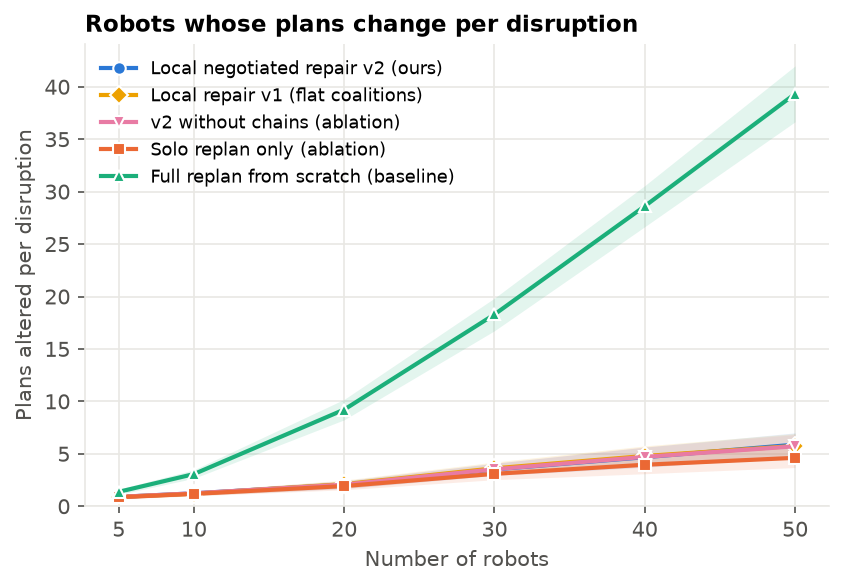
\includegraphics[width=\linewidth]{agents_altered.png}\end{subfigure}
  \begin{subfigure}{0.49\linewidth}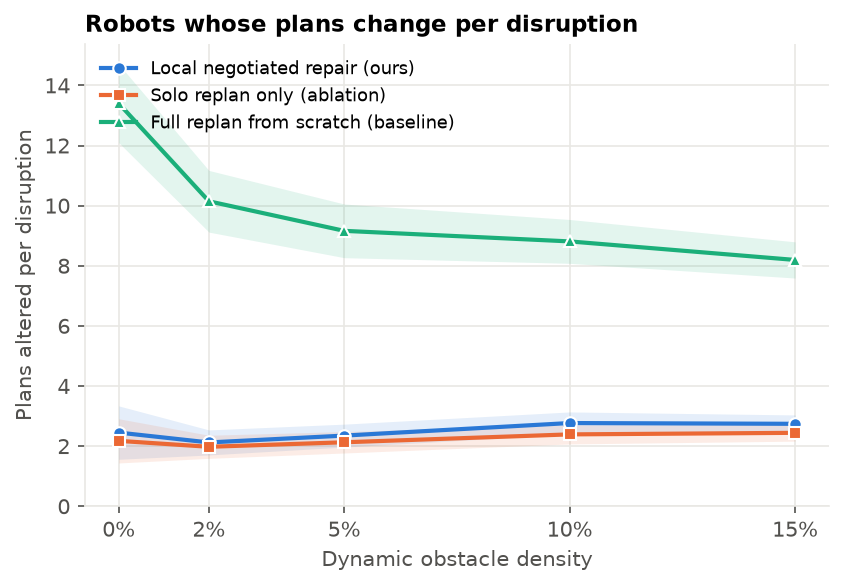
\includegraphics[width=\linewidth]{density_altered.png}\end{subfigure}
  \caption{How many robots change their plan per disruption, as the number of robots grows (left)
  and as obstacles get denser (right). Our method (blue) stays low; re-planning everything
  (green) changes almost the whole fleet.}
  \label{fig:altered}
\end{figure}

\textbf{Main findings.}
\begin{enumerate}\setlength{\itemsep}{2pt}
  \item \textbf{We change very few plans.} Our method changes about one robot more than the ones
        the disruption hits directly. Re-planning everyone changes 9 to 39 robots per disruption.
  \item \textbf{Re-planning everyone is not even faster.} At 50 robots its total time is
        \emph{worse} than ours (7201 vs 6958 steps), because it reshuffles all robots, including
        ones that were never affected.
  \item \textbf{One disruption, how many plans?} A temporary breakdown changes 2.2 plans (exactly
        the robots it blocks), a temporary blockage 3.1, and a permanent breakdown 13.5 (the
        broken robot's tasks are handed to others). Re-planning everyone changes 22 to 29
        (Figure~\ref{fig:single}, left).
  \item \textbf{Talking helps more as the fleet grows.} With 50 robots, fixing alone
        (\texttt{solo}) needs 131 more steps than our method.
  \item \textbf{Improvements over our first version.} Our final version has 7 to 19 fewer total
        steps at 30 to 50 robots and meets more emergency deadlines (35\% vs 15\% at 50 robots),
        while changing about as many plans. The price: repairs take about twice as long.
\end{enumerate}

\subsection*{How performance changes with more robots and denser obstacles}
Table~\ref{tab:scaling} lists every setting we tried. Figure~\ref{fig:soc} shows total time.

\begin{table}[H]
\centering\footnotesize\setlength{\tabcolsep}{4.5pt}
\caption{All results for both experiments (average of 10 runs). Top: number of robots
(3\% density). Bottom: obstacle density (20 robots; disruptions per run in brackets). ``Extra
steps'' is the time lost to disruptions. ``Plans altered'' and ``repair ms'' are per disruption.}
\label{tab:scaling}
\begin{tabular}{lrrrrrrrrr}
\toprule
 & \multicolumn{3}{c}{total time} & \multicolumn{2}{c}{extra steps} & \multicolumn{2}{c}{plans altered} & \multicolumn{2}{c}{repair ms}\\
\cmidrule(lr){2-4}\cmidrule(lr){5-6}\cmidrule(lr){7-8}\cmidrule(lr){9-10}
 & local & solo & full & local & full & local & full & local & full\\
\midrule
\multicolumn{10}{l}{\textit{Number of robots}}\\
5  robots & 679  & 681  & 679  & 108 & 109 & 0.89 & 1.38  & 3    & 5 \\
10 robots & 1330 & 1330 & 1332 & 146 & 148 & 1.23 & 3.07  & 5    & 10 \\
20 robots & 2612 & 2622 & 2611 & 190 & 189 & 2.06 & 9.22  & 126  & 41 \\
30 robots & 4093 & 4148 & 4131 & 252 & 290 & 3.52 & 18.29 & 416  & 124 \\
40 robots & 5510 & 5572 & 5617 & 345 & 452 & 4.68 & 28.62 & 1115 & 289 \\
50 robots & 6958 & 7089 & 7201 & 377 & 620 & 5.88 & 39.33 & 2270 & 590 \\
\midrule
\multicolumn{10}{l}{\textit{Obstacle density (disruptions per run)}}\\
0\% (4)   & 2565 & 2568 & 2555 & 143 & 133 & 2.52 & 13.40 & 70  & 45 \\
2\% (9)   & 2583 & 2591 & 2592 & 161 & 171 & 2.14 & 10.14 & 61  & 45 \\
5\% (18)  & 2630 & 2652 & 2629 & 208 & 208 & 2.34 & 9.16  & 112 & 62 \\
10\% (31) & 2768 & 2831 & 2813 & 347 & 392 & 2.63 & 8.81  & 247 & 116 \\
15\% (45) & 2925 & 2995 & 2997 & 503 & 575 & 2.74 & 8.20  & 320 & 1712 \\
\bottomrule
\end{tabular}
\end{table}

\begin{figure}[H]
  \centering
  \begin{subfigure}{0.49\linewidth}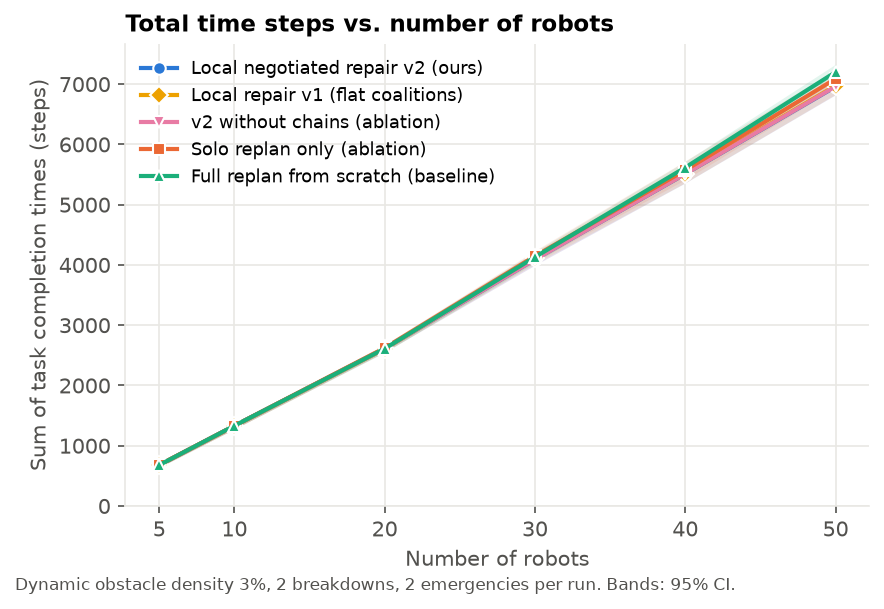
\includegraphics[width=\linewidth]{agents_soc.png}\end{subfigure}
  \begin{subfigure}{0.49\linewidth}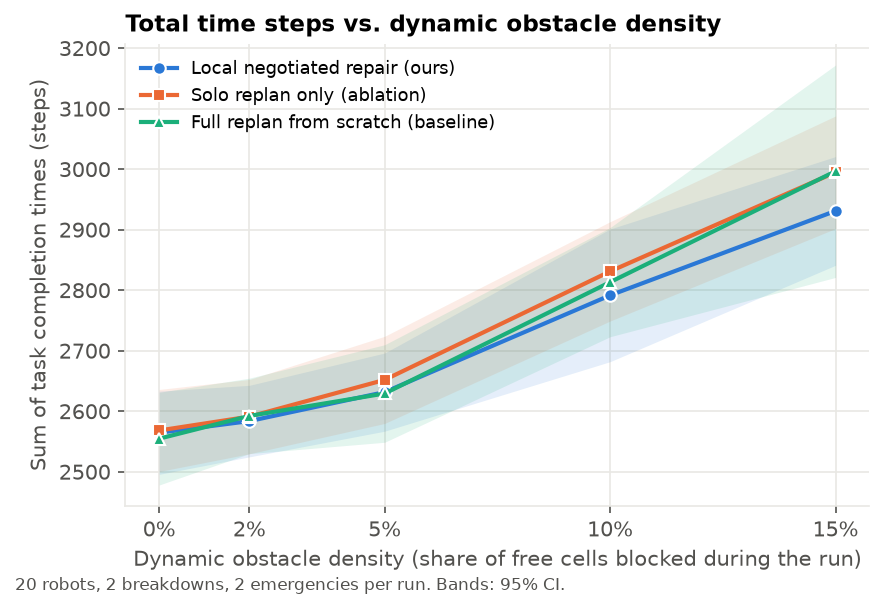
\includegraphics[width=\linewidth]{density_soc.png}\end{subfigure}
  \caption{Total time as the number of robots grows (left) and as obstacles get denser (right).
  Lower is better.}
  \label{fig:soc}
\end{figure}

\textbf{More robots.}
\begin{itemize}\setlength{\itemsep}{1pt}
  \item Total time grows in a straight line, about 140 steps per extra robot, because each robot
        brings 3 more tasks.
  \item The time \emph{lost} to disruptions grows faster, because a crowded floor has fewer
        detours: from 108 to 377 extra steps with our method, but up to 620 when re-planning
        everyone.
  \item Up to 20 robots all methods are about equal. From 30 robots on, ours is clearly best
        (37, 107 and 243 steps better than re-planning everyone at 30, 40 and 50 robots).
  \item Plans changed grow slowly for us (0.9 to 5.9) but almost one-for-one with the fleet when
        re-planning everyone (1.4 to 39).
  \item The cost is computing time: our repair takes 3\,ms with 5 robots and 2.3\,s with 50,
        because more neighbours means more groups to try.
\end{itemize}

\textbf{Denser obstacles.}
\begin{itemize}\setlength{\itemsep}{1pt}
  \item Going from 0\% to 15\% density means 4 to 45 disruptions per run, and our total time
        rises by 14\% (2565 to 2925). Each extra disruption costs about 9 steps.
  \item Plans changed per disruption stay almost the same (2.1 to 2.7), because a blocked cell
        only affects the few robots about to cross it.
  \item At low density all methods are within about 10 steps. From 10\% on, ours saves 45 to 72
        steps compared with re-planning everyone, and at 15\% re-planning everyone becomes slow
        (1.7\,s per disruption vs.\ our 0.3\,s).
\end{itemize}

\begin{figure}[H]
  \centering
  \begin{subfigure}{0.49\linewidth}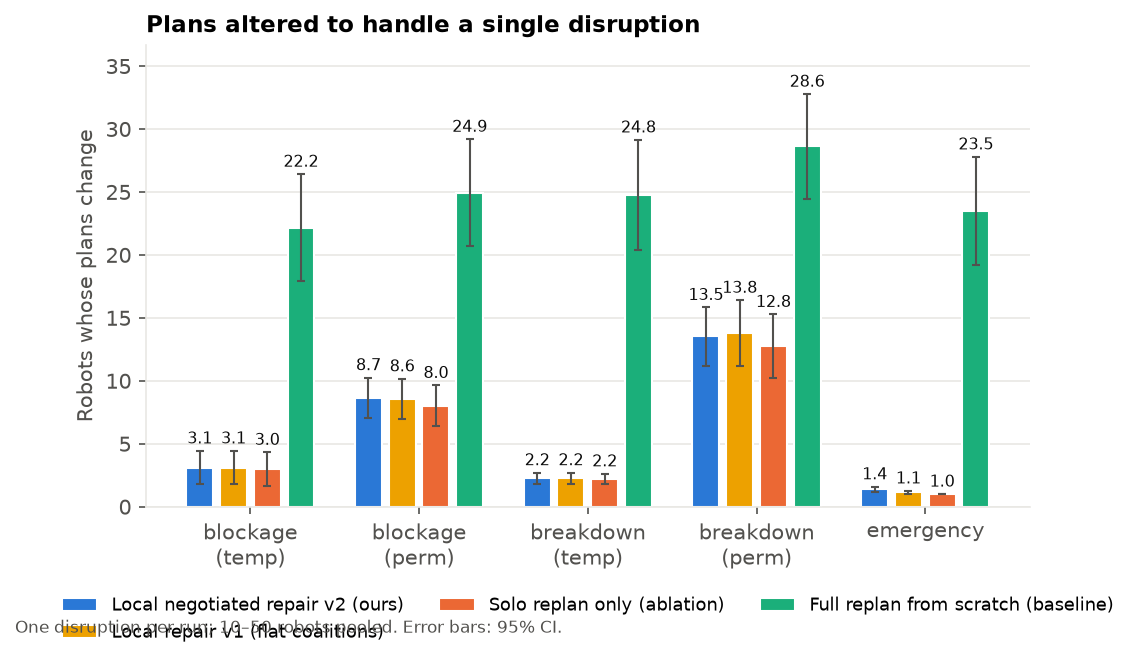
\includegraphics[width=\linewidth]{single_altered.png}\end{subfigure}
  \begin{subfigure}{0.49\linewidth}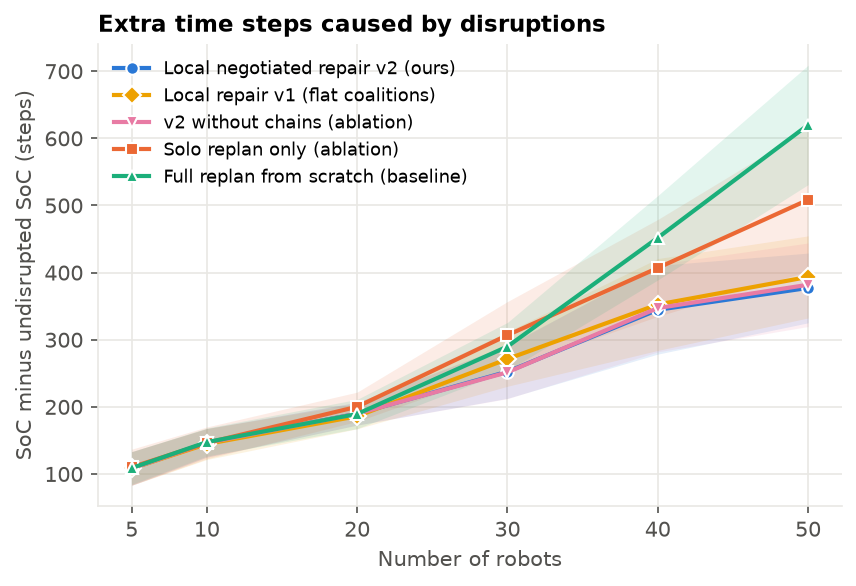
\includegraphics[width=\linewidth]{agents_overhead.png}\end{subfigure}
  \caption{Left: robots whose plans change after a \emph{single} disruption, per type. Right:
  steps lost to disruptions as the number of robots grows.}
  \label{fig:single}
\end{figure}

\textbf{The ``3 per robot'' setting.} The value 3 in the score decides the balance between
``disturb fewer robots'' and ``finish faster''. Figure~\ref{fig:lambda} shows what happens for other
values (0 to 12): a small value finishes a little faster but disturbs more robots; a large value
does the opposite. We chose 3 as a middle ground.

\begin{figure}[H]
  \centering
  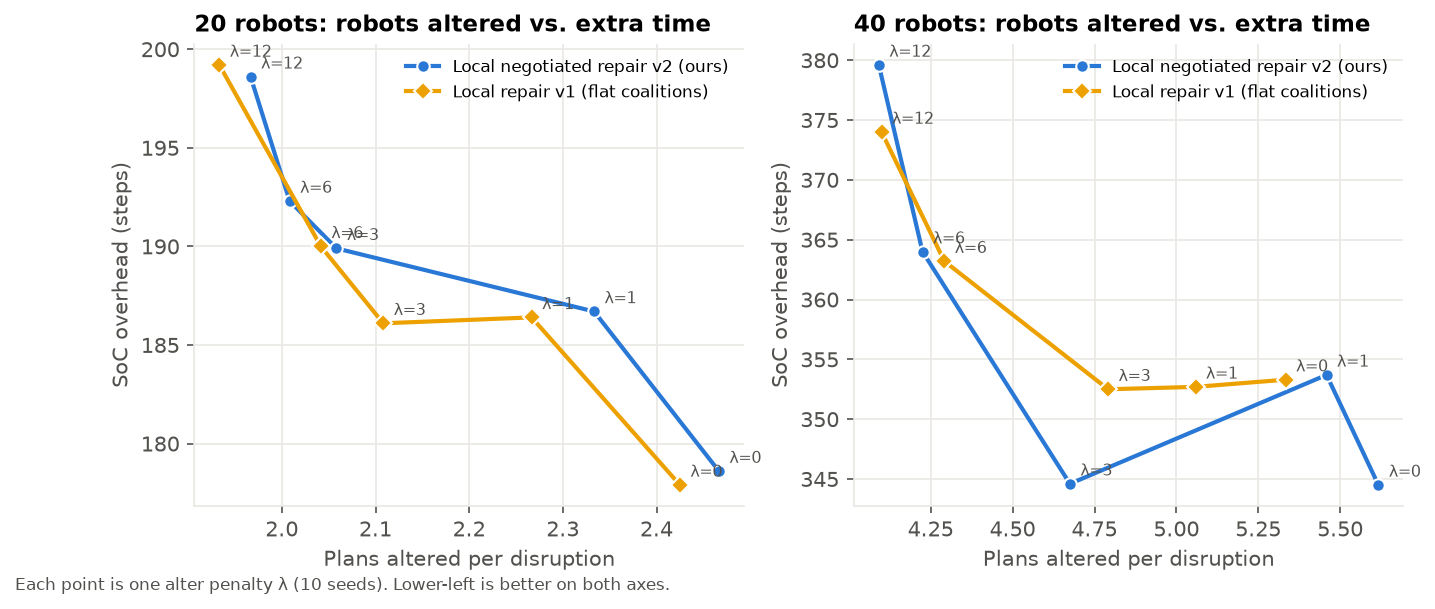
\includegraphics[width=0.72\linewidth]{lambda_tradeoff.png}
  \caption{Trade-off between robots disturbed (x-axis) and steps lost (y-axis) for different values
  of the per-robot penalty $\lambda$. Points further down and to the left are better.}
  \label{fig:lambda}
\end{figure}

\inshort{our method changes only a few plans per disruption, no matter how many robots or obstacles
there are, and it is as fast or faster than re-planning everyone. Its cost is computing time,
which grows with the number of robots.}

\section{When do the robots fail?}
\label{sec:fail}
In our normal tests the robots almost never fail. One reason is that our test generator never
creates impossible situations: for example, it never blocks a cell that would wall off a goal. To
find out where things break, we ran a \textbf{stress test} (760 runs) in which we turned that safety
filter off and pushed the warehouse harder. A run \textbf{fails} if some task is never finished. For
each robot that gets stuck we record why:
\begin{itemize}\setlength{\itemsep}{1pt}
  \item \textbf{goal cut off}: its goal can no longer be reached at all (the task became impossible);
  \item \textbf{deadlocked}: its goal \emph{can} be reached, but the robot is stuck waiting.
\end{itemize}

\begin{figure}[H]
  \centering
  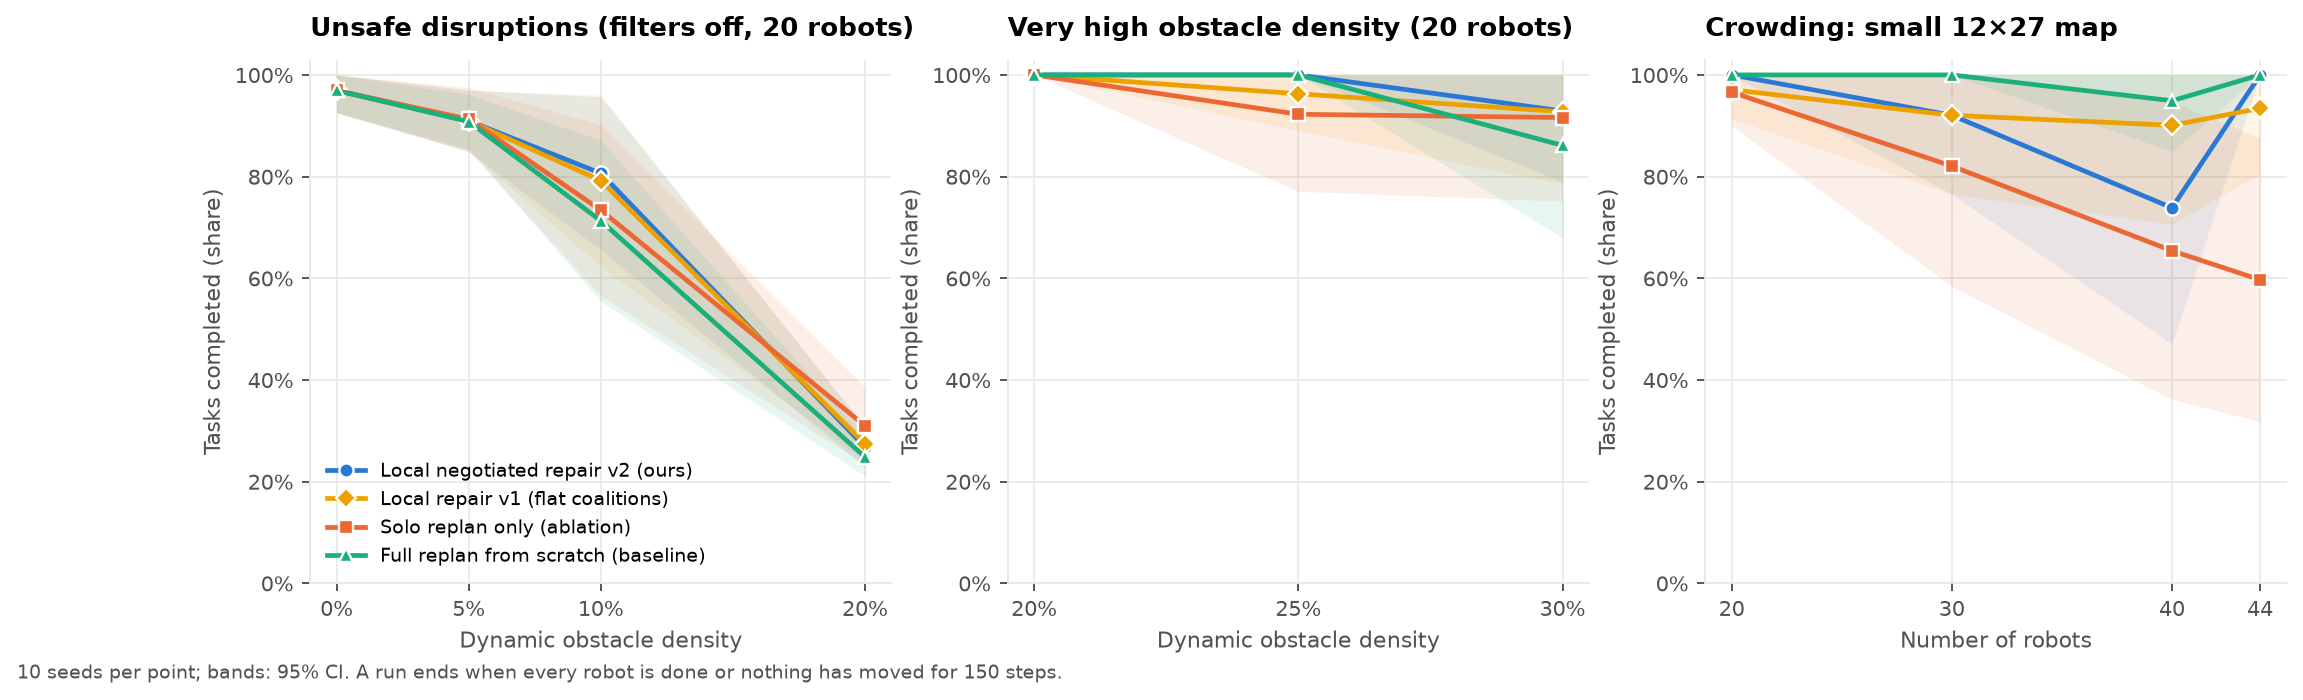
\includegraphics[width=\linewidth]{stress_completion.png}
  \caption{Share of tasks completed in each stress setting. 100\% means every task was done.}
  \label{fig:stress}
\end{figure}

\begin{table}[H]
\centering\footnotesize\setlength{\tabcolsep}{4pt}
\caption{Where the robots fail. ``Failed'' = runs (out of 10) with an unfinished task.
``Stuck'' = average stuck robots per run with our method (goal cut off / deadlocked).}
\label{tab:fail}
\begin{tabular}{llrrrrr}
\toprule
 & & \multicolumn{3}{c}{\texttt{local} (ours)} & \texttt{local-flat} & \texttt{full}\\
\cmidrule(lr){3-5}\cmidrule(lr){6-6}\cmidrule(lr){7-7}
setting & value & failed & completed & stuck: cut / dead & completed & completed\\
\midrule
filter off,          & density 0\%  & 3/10  & 96.9\% & 0.5 / 0.2 & 96.9\% & 96.9\% \\
half of the events   & density 5\%  & 7/10  & 91.0\% & 1.5 / 0.3 & 91.0\% & 90.8\% \\
are permanent        & density 10\% & 10/10 & 80.6\% & 2.3 / 3.1 & 79.2\% & 71.3\% \\
                     & density 20\% & 10/10 & 26.8\% & 9.9 / 8.8 & 27.4\% & 24.8\% \\
\midrule
one permanent breakdown, & 20 robots & 2/10 & 97.5\% & 0.4 / 0.2 & 97.5\% & 97.5\% \\
filter off               & 40 robots & 4/10 & 96.7\% & 0.4 / 1.0 & 96.7\% & 96.7\% \\
\midrule
very dense obstacles, & density 25\% & 0/10 & 100\%  & --        & 96.3\% & 100\% \\
filter on             & density 30\% & 1/10 & 92.9\% & 0.0 / 2.0 & 92.7\% & 86.1\% \\
\midrule
crowded small map     & 30 robots & 1/10 & 92.1\% & 0.0 / 2.9  & 92.1\% & 100\% \\
($12\times27$ cells)  & 40 robots & 3/10 & 73.9\% & 0.0 / 11.9 & 90.1\% & 94.9\% \\
                      & 44 robots & 0/10 & 100\%  & --         & 93.4\% & 100\% \\
\midrule
short talking range (40 robots) & 1, 2, 3, 6 cells & 0/10 & 100\% & -- & 100\% & 100\% \\
\bottomrule
\end{tabular}
\end{table}

\begin{figure}[H]
  \centering
  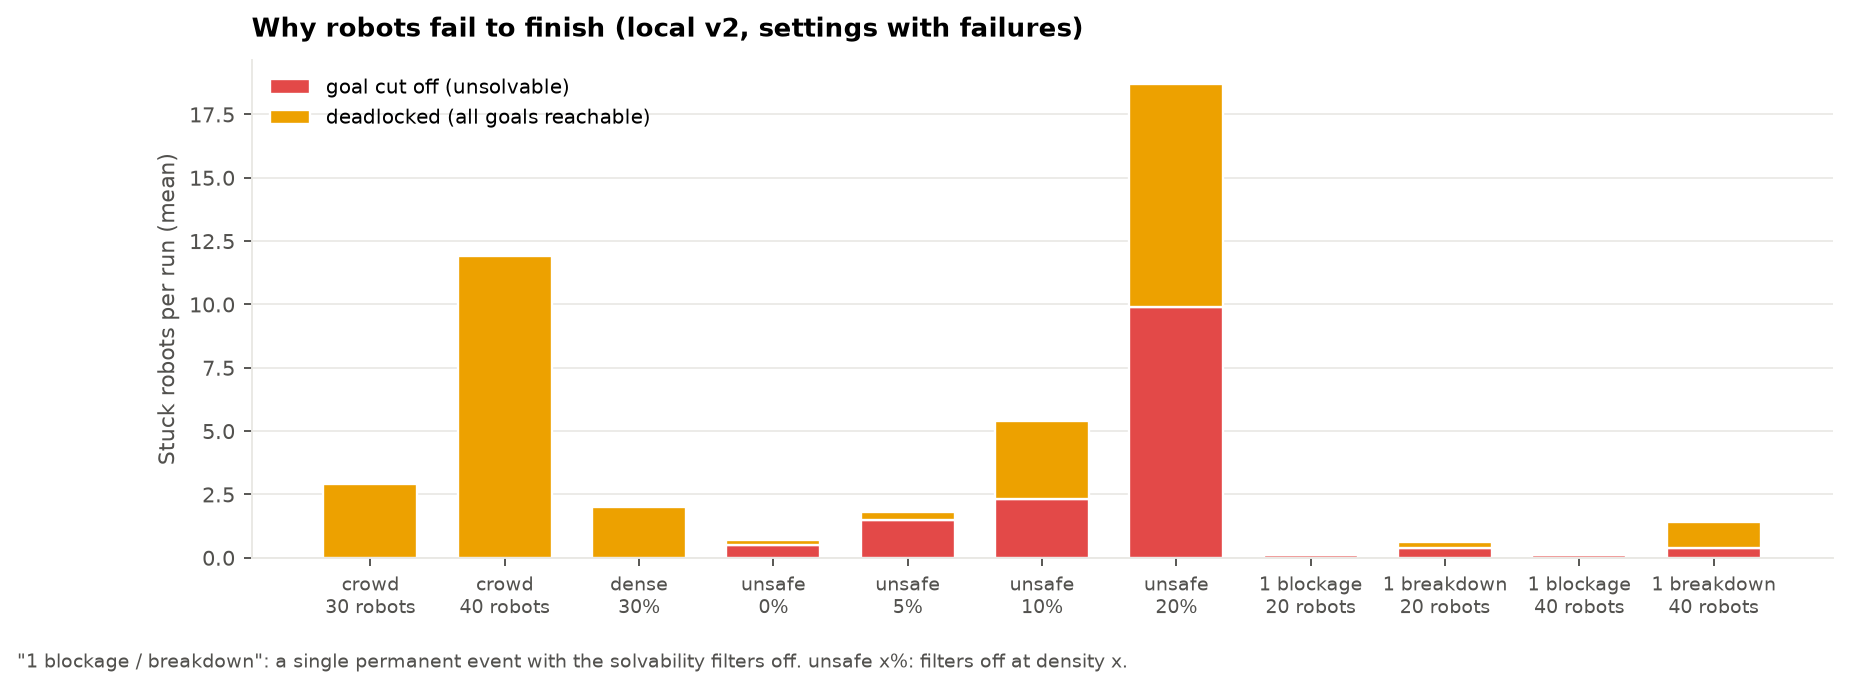
\includegraphics[width=0.8\linewidth]{stress_causes.png}
  \caption{Why robots get stuck with our method. Red: the goal was cut off. Orange: deadlocked,
  even though the goal could still be reached.}
  \label{fig:causes}
\end{figure}

\textbf{1. Goals get cut off.} When a cell is blocked for good, or a robot breaks down for good in
a one-cell-wide aisle, it can wall off a pickup cell or a station (Figure~\ref{fig:unreach}). Then no
method can finish that task, so all methods fail in the same way. Completion falls from 97\% to
27\% as the density goes up to 20\%. Even a single robot breaking down for good makes 2 to 4 out of
10 runs fail.

\textbf{2. Stuck robots block others.} A robot whose goal is cut off never gives up. It keeps
waiting in its cell, and that cell may be the only way through for other robots. At 10\% density,
2.3 robots per run have their goal cut off, but another 3.1 get stuck \emph{behind} them. So more
than half of the stuck robots are caused by how the robots react, not by the task being
impossible. Our method still does better here than re-planning everyone (81\% vs 71\% completed).

\textbf{3. Waiting spreads on a crowded map (our main weakness).} On a small map with 40 robots,
3 of 10 runs fail with almost every robot stuck. Example: a robot breaks down for just a few steps
and blocks 6 robots, which start waiting. Robots that planned to pass through a waiting robot's cell
then wait too, and so on, until all 40 robots are waiting for each other. Only 1 of 122 tasks gets
done. Our groups are too small (at most 4 or 8 robots) to untangle this, while re-planning everyone
solves it. This depends on the exact situation: with 44 robots, no run failed.

\begin{figure}[H]
  \centering
  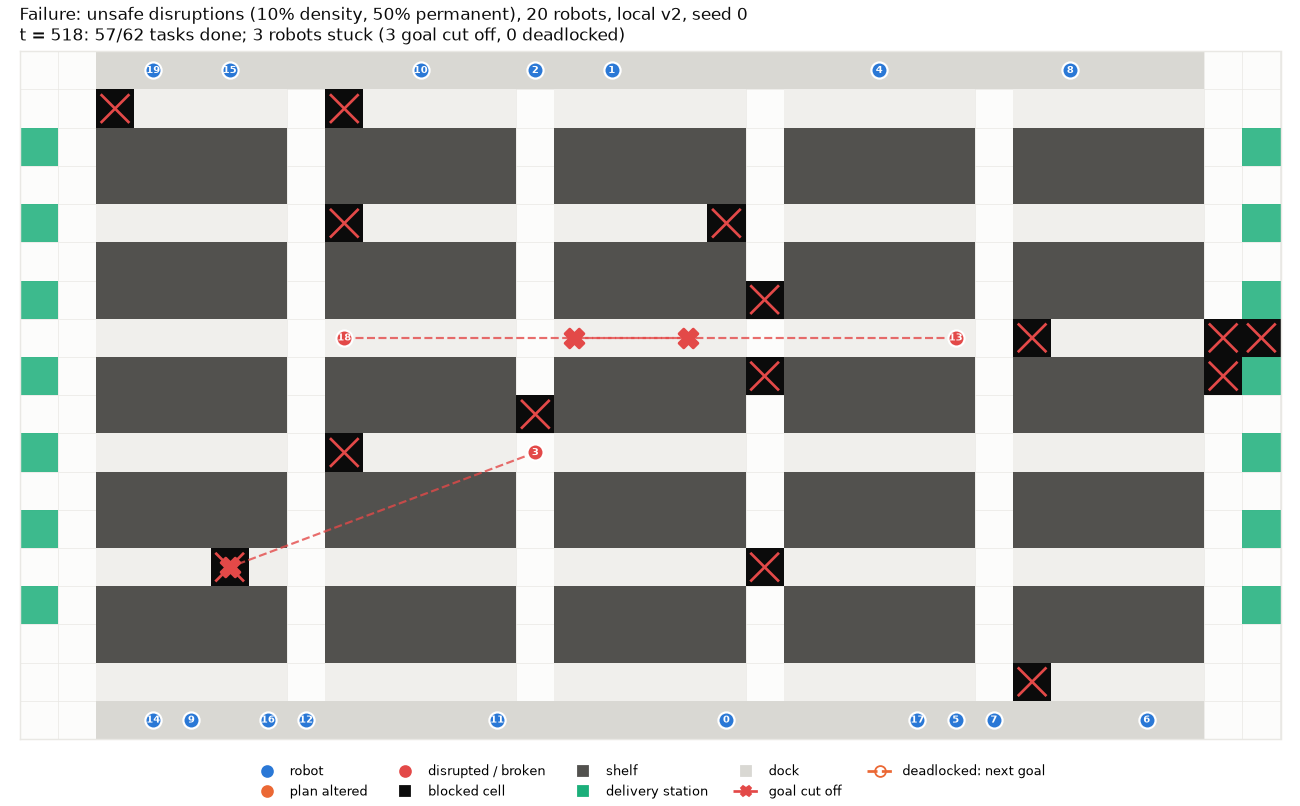
\includegraphics[width=0.66\linewidth]{failure_unreachable.png}
  \caption{Failure example: permanently blocked cells (black) cut off the goals of robots 3, 13
  and 18 (red). 5 of 62 tasks are never done.}
  \label{fig:unreach}
\end{figure}

\textbf{4. Other cases.}
\begin{itemize}\setlength{\itemsep}{1pt}
  \item \textbf{Very dense obstacles:} at 30\% density (all tasks still possible), 1 of 10 runs
        gets a deadlock.
  \item \textbf{No talking:} without negotiation (\texttt{solo}), all 49 remaining robots got
        stuck after one robot broke down for good with 50 robots (Figure~\ref{fig:gridlock}), and
        5 of 10 runs failed on the crowded map. Our method solved both.
  \item \textbf{Emergency deadlines:} in crowded warehouses only 5--35\% of emergency deliveries
        are on time, although all of them are eventually delivered.
\end{itemize}
\textbf{Where they did \emph{not} fail:} with a very short talking range (even 1 cell, it costs only
1\% more time, because a robot that waits too long starts asking robots further away), and in any
normal (solvable) test with up to 50 robots and 20\% density.

\begin{figure}[H]
  \centering
  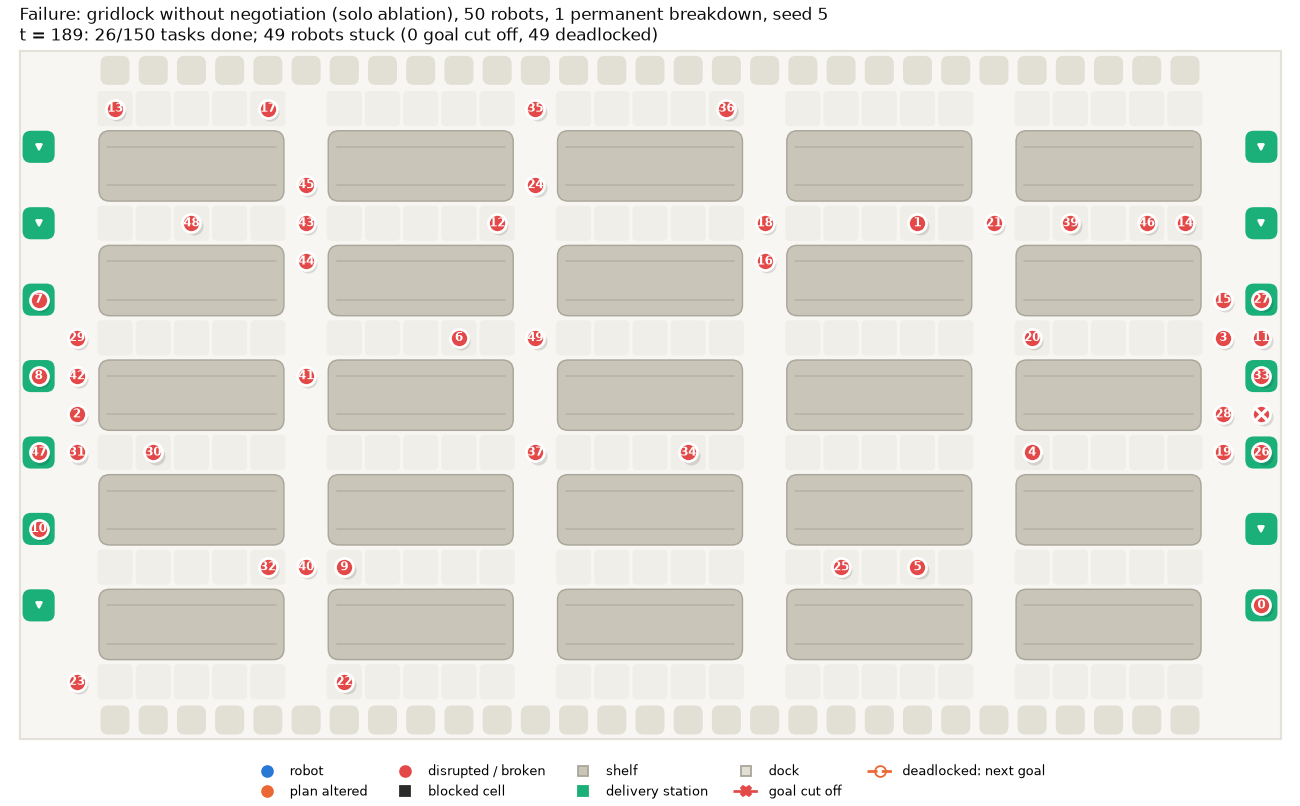
\includegraphics[width=0.66\linewidth]{failure_gridlock_solo.png}
  \caption{Failure without talking (\texttt{solo}): after one permanent breakdown, all 49 remaining
  robots (red) wait for each other forever. Our method finishes all 150 tasks in the same situation.}
  \label{fig:gridlock}
\end{figure}

\inshort{robots fail when (1) a goal becomes unreachable, (2) a stuck robot blocks others, (3) waiting
spreads through a very crowded map, (4) obstacles are extremely dense, or (5) robots cannot talk to
each other.}

\section{Graphical demonstration}
We made the simulations with Python's matplotlib library:
\begin{itemize}\setlength{\itemsep}{1pt}
  \item an \textbf{MP4 video} of 20 robots handling 12 disruptions (one frame in Figure~\ref{fig:demo});
  \item \textbf{before/after pictures} of each type of disruption (old plan dashed, new plan solid);
  \item \textbf{videos of the failure cases} from Section~\ref{sec:fail};
  \item an \textbf{interactive replay} in the browser and a live replay window.
\end{itemize}
For a few steps after each disruption, the video colours the robots whose plans changed in orange
and draws their new paths.

\begin{figure}[H]
  \centering
  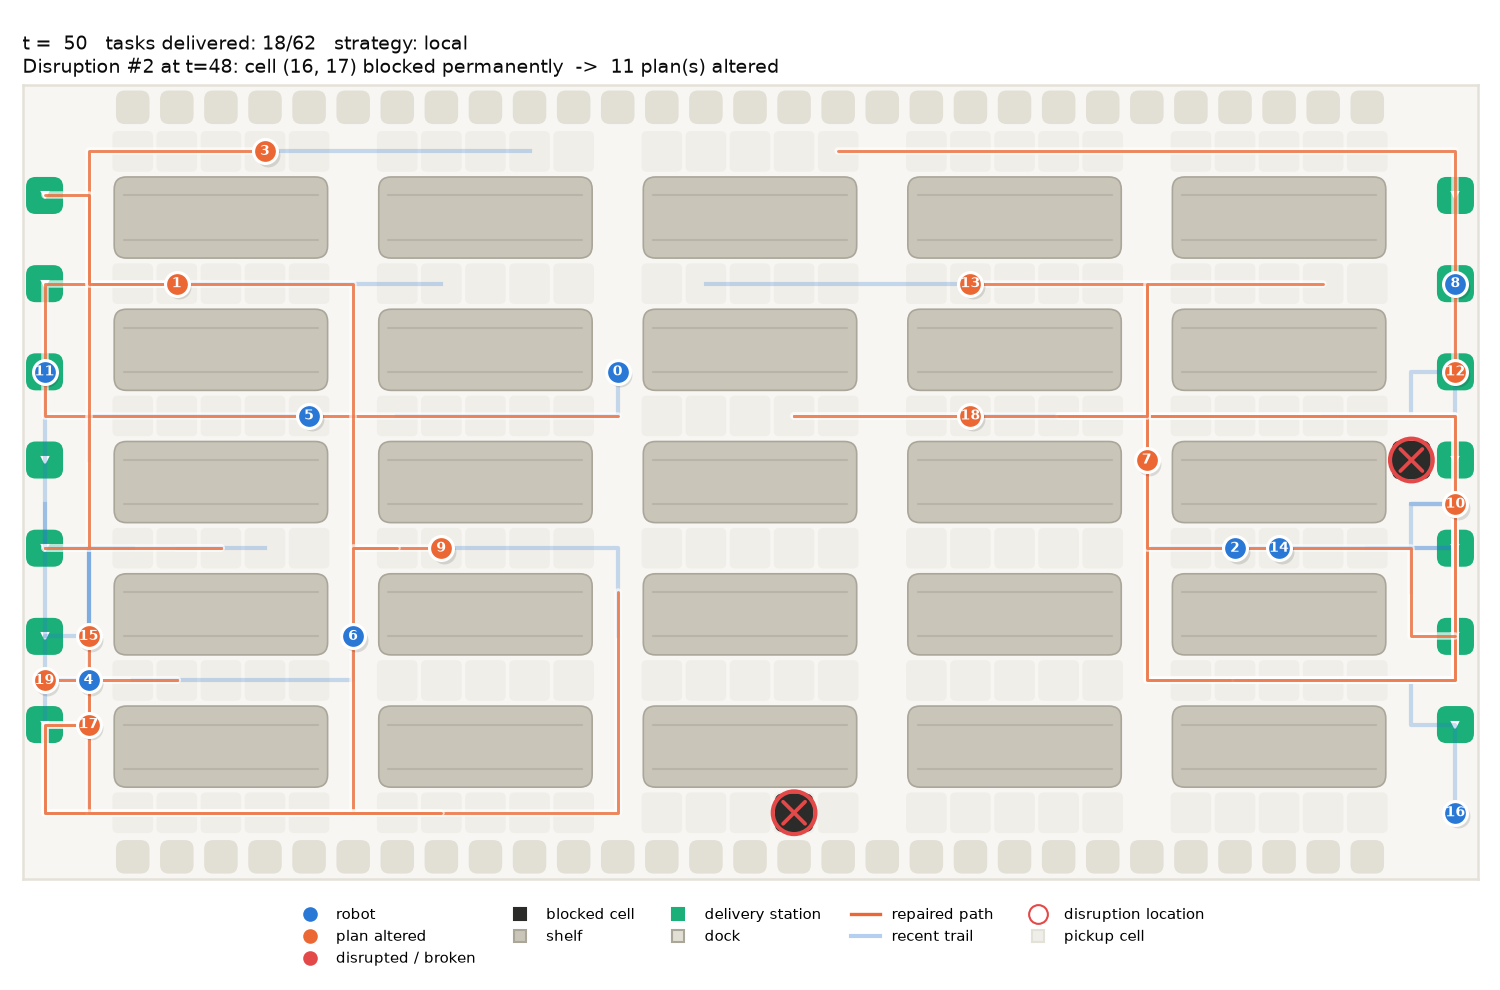
\includegraphics[width=0.7\linewidth]{demo_frame.png}
  \caption{A frame from the video, just after a cell was blocked for good (red circle). 11 robots
  changed their plans: they are orange, and the orange lines are their new paths.}
  \label{fig:demo}
\end{figure}

\section{Limitations}
\begin{itemize}\setlength{\itemsep}{1pt}
  \item \textbf{Planning one robot at a time is not perfect:} it can fail to find a plan even when
        one exists.
  \item \textbf{Robots never give up a task:} a robot whose goal is cut off waits forever and can
        block others.
  \item \textbf{Waiting can spread on crowded maps:} a fix would be to re-plan a bigger area when
        many robots start waiting.
  \item \textbf{Emergency deadlines are soft:} missing one only adds a penalty, so in crowded
        warehouses most are missed.
  \item \textbf{Repairs get slow with many robots:} about 2 seconds per disruption at 50 robots in
        Python.
  \item \textbf{Perfect communication is assumed:} messages arrive instantly and are never lost.
\end{itemize}

\vspace{4pt}
\noindent\textbf{Code, results and demos:} \url{https://github.com/SreenityaThatikunta/warehouse-plan-repair}

\end{document}
